\chapter{Results}
\label{chap:results}

% \begin{itemize}
%     \item Average precision
%     \begin{itemize}
%         \item Main set of categories
%         \item Small set of categories
%         \item Skiing classification
%     \end{itemize}
%     \item Precision-recall curves
%     \begin{itemize}
%         \item Main set of categories
%         \item Small set of categories
%         \item Skiing classification
%     \end{itemize}
%     \item Dataset analysis
%     \begin{itemize}
%         \item Number of categories, pictures
%         \item Number of labels per picture
%         \item Top categories
%         \item Examples of Norwegian-specific categories
%         \item Examples of news-agency specific content
%     \end{itemize}
%     \item Categories tree evaluation
%     \begin{itemize}
%         \item Examples of context, double-meaning, vague labels
%         \item Examples of different children-parent relationship
%         \item Different types of labels: objects, events, state, action etc.
%         \item Granularity of categories
%     \end{itemize}
%     \item AP improvement when removing faces from sports (GTX 580 only)
%     \item Comparison of precision-recall curves of different categories
%     \item Comparison of AP for different iterations
%     \item Adam vs SGD solvers on GTX 580, small category list
%     \item Training speed comparison for Titan and GTX 580 (but CPU and SSD can also contribute)
%     \item Different split techniques
%     \item Network performance on ImageNet images* (not done yet)
% \end{itemize}


\section{Dataset analysis}
Results of the initial analysis of the dataset provided by NTB are presented in this section. This analysis was the basis for the further experiments design and implementation.

NTB categories are organized in a tree structure that contains 3006 nodes. There are 31 top-level categories, which are shown in Table \ref{table:top-level-categories}. This table also contains a number of descendants each top-level category has, as well as a total number of pictures that belong to this category subtree.  Each image can belong to zero or more categories, meaning that categories were not designed to be mutually exclusive on any level of the categories tree. Top 20 categories with the most pictures in them are shown on the Figure \ref{fig:top-cats-distribution}. Provided NTB dataset contains 912324 of images, 805946 (88\%) of them have at least one label, therefore belong at least to one category. The whole category tree is too big to visualize it in any way, however, the most important highlights and insights are provided further in this section.

\begin{table}[h!]
    \centering
    \csvautotabular[respect sharp]{tables/top-level-categories.csv}
    \caption{Top Level categories with total number of descendants and images}
    \label{table:top-level-categories}
\end{table}

\begin{figure}[h!]
    \centering
    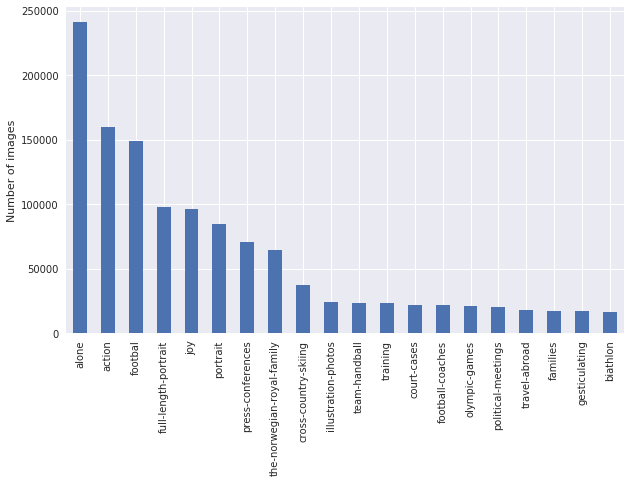
\includegraphics[width=0.9\textwidth]{top-cats-distribution}
    \caption{Distribution of images in top 20 categories}
    \label{fig:top-cats-distribution}
\end{figure}

From both Table \ref{table:top-level-categories} as well as Figure \ref{fig:top-cats-distribution} it is possible to see that the provided dataset is focused on sports, politics and finance topics, which is expected since NTB is a Norwegian news content providing company. Further analysis also shows that many categories are specific to Norway, for example \textit{norwegian-royal-family}, \textit{cross-country-skiing}, \textit{the-king's-throne-speech}, \textit{the-parliament-building}, \textit{stave-churches}, \textit{norwegian-national-costumes} etc. The category types are also very diverse. For example there are categories which represent simple objects (\textit{tv-sets}, \textit{cars}, \textit{doors}), abstractions (\textit{communism}, \textit{neo-nazism}), group of people (\textit{policemen}, \textit{politicians}, \textit{christians}), holidays (\textit{christmas}, \textit{national-days}), relationships (\textit{grandchildren}, \textit{daughters}), sports (\textit{skiing}, \textit{football}), actions (\textit{handshake}, \textit{document-signing}) etc.

Figure \ref{fig:num-labels} illustrate the distribution of the number of labels per one image in the dataset. Most of the images have from two to four labels associated with them. This fact together with the non-mutual exclusive set of categories, as well as the real-world nature of the images (which potentially are more crowded), makes a multi-label classification system more suitable for this dataset than a single-label. There is a label \textit{alone} in the NTB set of categories that is used to identify images which contain a single object. This label should not be confused with a single-label case of classification since even if there is only one object on the picture, in the multi-label case it can belong to several categories which describe this object. For example, even though figures \ref{fig:without-sign-of-triumph} and \ref{fig:with-sign-of-triumph} both contain label \textit{alone}, they both also contain number of other labels that describe these pictures in different dimensions (kind of sport, gender, emotions etc).

\begin{figure}[h!]
    \centering
    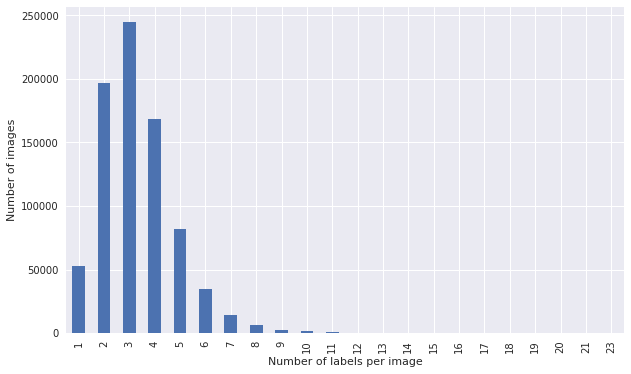
\includegraphics[width=0.9\textwidth]{num-labels}
    \caption{Number of labels per one image distribution}
    \label{fig:num-labels}
\end{figure}

Analysis of the categories tree, as well as example images from different categories, revealed some issues connected with the dataset described further.

\paragraph{Mistakes and not visible entities}
In many cases labeled object on the picture is not located in the center or even clearly visible. For example, picture labeled as \textit{blueberries} is shown on Figure \ref{fig:image-blueberries}. No blueberries are visible on this image, the main entity visualized on the picture is the person. However, the image is not even labeled with the tag \textit{person}.

\begin{figure}[h]
    \centering
    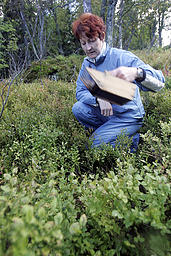
\includegraphics[width=0.4\textwidth]{images/sp616962}
    \caption[Example picture from the \textit{blueberries} category]{\textit{blueberries}, \textit{berries}, \textit{autumn}, \textit{illustration-photos}. Photo by Terje Bendiksby~/~Scanpix}
    \label{fig:image-blueberries}
\end{figure}

\paragraph{Not consistent labels}
Some labels are not consistent across the whole dataset. For example, \textit{sign-of-triumph} label is applied on images that have person with two hands raised up. However, often this label is missing on images and only label \textit{joy} is applied. This issue is illustrated on Figure \ref{fig:sign-of-triumph-example}, where from two visually similar images only one has \textit{sign-of-triumph} label.

\begin{figure}[ht]
    \centering
    \begin{subfigure}[a]{0.3\textwidth}
        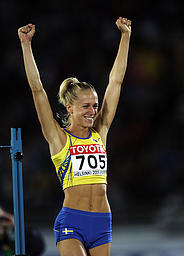
\includegraphics[width=\textwidth]{images/sp8718f2}
        \caption{\textit{alone}, \textit{athletics}, \textit{high-jump}, \textit{women}, \textit{sign-of-triumph}, \textit{joy}. Photo by Cornelius Poppe~/~Scanpix}
        \label{fig:with-sign-of-triumph}
    \end{subfigure}
    ~
    \begin{subfigure}[a]{0.3\textwidth}
        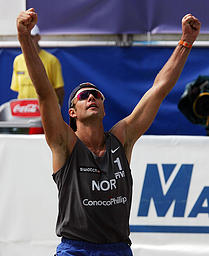
\includegraphics[width=\textwidth]{images/sp525daa}
        \caption{\textit{alone}, \textit{beach-volleyball}, \textit{action}, \textit{joy}. Photo by Alf Ove Hansen~/~Scanpix}
        \label{fig:without-sign-of-triumph}
    \end{subfigure}
    \caption[Example of two similar images and with different labels]{Example of two similar images and with different labels. Only one image belongs to \textit{sign-of-triumph} category}
    \label{fig:sign-of-triumph-example}
\end{figure}

\paragraph{Different purpose of labels}
Labels in the NTB dataset can have a different purpose. Most of the labels define some entity or action that is presented in the picture. However, some labels are designed to be a modification of other labels. For example, label \textit{action} was designed to be used together with any sports category like \textit{football} to get football players in action. Mentioned earlier label \textit{alone} serves to identify images withing particular category with only one object illustrated on them. This inconsistency can potentially influence resulting classification system performance.

\paragraph{Contextual categories}
There are many contextual categories, where visual information is not enough to determine if image should belong to the category and additional context information is necessary. Example of such categories: \textit{second-hand-cloth}, \textit{used-cars}, \textit{counterfeit-money}, \textit{finance-debates}. More issues discovered during category tree evaluation are presented in section \ref{sec:tree-eval}.

\paragraph{Contextual images}
There are many images which have an assigned category that can not be derived only from the image itself and more contextual information is needed. For example, picture that is part of the category \textit{politicians} as well as \textit{fishfarming} and \textit{fisheries-industry} is shown on Figure \ref{fig:politician-fish}. While the first category can potentially be automatically derived using face-recognition approach, the second and the third categories are fully contextual. In order to assign these labels to the picture, the system needs more additional information such as when and where the picture was taken as well as what was discussed in this place and time. Another example is press-conference or portrait pictures that are part of some sports category. From 151533 images of football, 151533 (10.4\%) belong to the \textit{coaches}, \textit{press-conferences} or \textit{portrait} categories as well.

\begin{figure}[h]
    \centering
    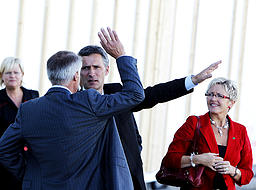
\includegraphics[width=0.6\textwidth]{images/sy253353}
    \caption[Example of contextual labeled images]{\textit{politicians}, \textit{fishfarming}, \textit{fisheries-industry}, \textit{travel-in-norway}. Photo by Gorm Kallestad / Scanpix}
    \label{fig:politician-fish}
\end{figure}

The reason for all of the mentioned issues can potentially be that the dataset, as well as its categories tree, were not designed for future automated classification system training. They, however, can influence negatively such system performance. Further sections of this thesis will try to address and discuss these discovered issues from the perspective of a creation of multi-label image classification system.

The size and uniqueness of the NTB dataset make it perfect subject of the research on real-world datasets that were not originally designed for automatic classification training and can be used to find possible solutions for presented issues that can also exist in other datasets of this kind. Broad, diverse and unique set of NTB categories also eliminates the possibility to direct use of the systems trained on a more standard set of categories like ImageNet. Therefore, training system on a new set of categories should be performed.

% Pictures total:  912324
% With tags:  805946
% Multiple tags: 93.5%

\section{Trial experiment}
    \subsubsection{Classification performance}
    \subsubsection{Adam vs SGD}
    \subsubsection{LMDB vs Python DataLayer}
    \subsubsection{Context improvements}
    % removing portraits

\section{Main experiment}
    \subsubsection{Dataset split method}
    \label{sec:split-comparison}
    % smart way vs straitforward
    \subsubsection{Classification performance}
    \subsubsection{Category tree evaluation and improvement}
    \label{sec:tree-eval}
